\subsection{Training}
\begin{frame}{Training Pipeline}
    \begin{itemize}
        \item \textbf{Objective}: Train a denoising diffusion model (DDIM U-Net) on grayscale images
        \item \textbf{Main Components}:
              \begin{enumerate}
                  \item Data Augmentation
                  \item DataLoader
                  \item Model Compilation
                  \item Training loop with mixed-precision
              \end{enumerate}
    \end{itemize}
\end{frame}


\begin{frame}{Compiling the Model}
    \begin{itemize}
        \item \textbf{Why}: optimize the model for better performance
        \item \textbf{Usage}:
              \begin{semiverbatim}
                  \texttt{model = torch.compile(model)}
              \end{semiverbatim}
        \item \textbf{Benefits}: improved batch throughput
    \end{itemize}
\end{frame}


\begin{frame}{Mixed-Precision with AMP}
    \begin{itemize}
        \item \textbf{GradScaler amd autocast}:
              \begin{itemize}
                  \item \texttt{GradScaler} for scaling gradients
                  \item \texttt{autocast} for automatic mixed precision
              \end{itemize}
        \item Reduce memory usage and speed up training
    \end{itemize}
\end{frame}

\begin{frame}{Training Loop}
    \begin{enumerate}
        \item Start the training \texttt{model.train()}
        \item For each epoch:
              \begin{itemize}
                  \item Move images to GPU (if available)
                  \item Generate noise and timesteps
                  \item Compute noise prediction on the input data
                  \item Prediction + MSE loss
                  \item Optimization + \texttt{scheduler.step()}
              \end{itemize}
        \item Save samples to visualize the model performance during training
        \item Compute and log average losses
        \item Save model weights each epoch
    \end{enumerate}
\end{frame}

\begin{frame}{Checkpointing}
    \begin{itemize}
        \item \textbf{Validation}:
              \begin{itemize}
                  \item \texttt{model.eval()} to set the model to evaluation mode
              \end{itemize}
        \item \textbf{Checkpoint}:
              \begin{itemize}
                  \item Save the model weights to a \texttt{.pth} file
                  \item Update loss, PSNR and SSIM history in \texttt{history.txt}
              \end{itemize}
        \item Monitor train vs validation loss over epochs aswell as PSNR and SSIM between the generated and original images
              \begin{itemize}
                  \item For each epoch sample 10 images from the validation set and compute the metrics
              \end{itemize}
    \end{itemize}
\end{frame}

\begin{frame}{Epochs Validation}
    \begin{itemize}
        \item \textbf{Metrics}:
              \begin{itemize}
                  \item PSNR: Peak Signal-to-Noise Ratio
                  \item SSIM: Structural Similarity Index
              \end{itemize}
        \item \textbf{Sample Generation}:
              \begin{itemize}
                  \item Pure noise sampling using DDIM scheduler
                  \item Validation reconstruction:
                        \begin{itemize}
                            \item Add noise to clean validation images
                            \item Model predicts and removes the noise
                        \end{itemize}
              \end{itemize}
        \item \textbf{Quality Assessment}:
              \begin{itemize}
                  \item PSNR range: 20-40 dB (higher = better reconstruction)
                  \item SSIM range: 0-1 (closer to 1 = better similarity)
                  \item Average metrics computed over 5-10 validation samples
              \end{itemize}
    \end{itemize}
\end{frame}
\begin{frame}{Monitoring Produced Samples}
    \begin{itemize}
        \item \textbf{Pure Noise Sampling}:
              \begin{itemize}
                  \item Tests model's ability to generate images from noise that are similar to the training data
                  \item Uses DDIM scheduler for iterative denoising
                  \item Saves generated images as \texttt{epoch\_\{epoch\}.png}
              \end{itemize}
        \item \textbf{Validation Reconstruction}:
              \begin{itemize}
                  \item Adds noise to clean validation images
                  \item Model predicts and removes the noise
                  \item Direct assessment of denoising performance
                  \item Saves reconstructed images as \texttt{reconstructed\_\{epoch\}.png}
              \end{itemize}
        \item \textbf{History Tracking}:
              \begin{itemize}
                  \item All metrics saved to \texttt{history.txt}
                  \item Enables trend analysis and model comparison
              \end{itemize}
    \end{itemize}
\end{frame}

\begin{frame}{Plots}
    \begin{itemize}
        \item \textbf{Loss Monitoring}:
              \begin{itemize}
                  \item Training vs Validation Loss curves over epochs
                  \item MSE loss
              \end{itemize}
        \item \textbf{Quality Metrics Visualization}:
              \begin{itemize}
                  \item PSNR trends with average values
                  \item SSIM trends with average values
                  \item Both metrics computed on validation reconstructions
                  \item Useful to track model performance
              \end{itemize}
    \end{itemize}
\end{frame}

\begin{frame}{Comprehensive Monitoring}
    \begin{itemize}
        \item \textbf{Comprehensive Monitoring}:
              \begin{itemize}
                  \item Three-panel subplot: Loss, PSNR, SSIM (as shown in the Figure \ref{fig:training_results})
                  \item Data read from \texttt{history.txt} file
                  \item Enables performance trend analysis
              \end{itemize}
    \end{itemize}
    \begin{figure}
        \centering
        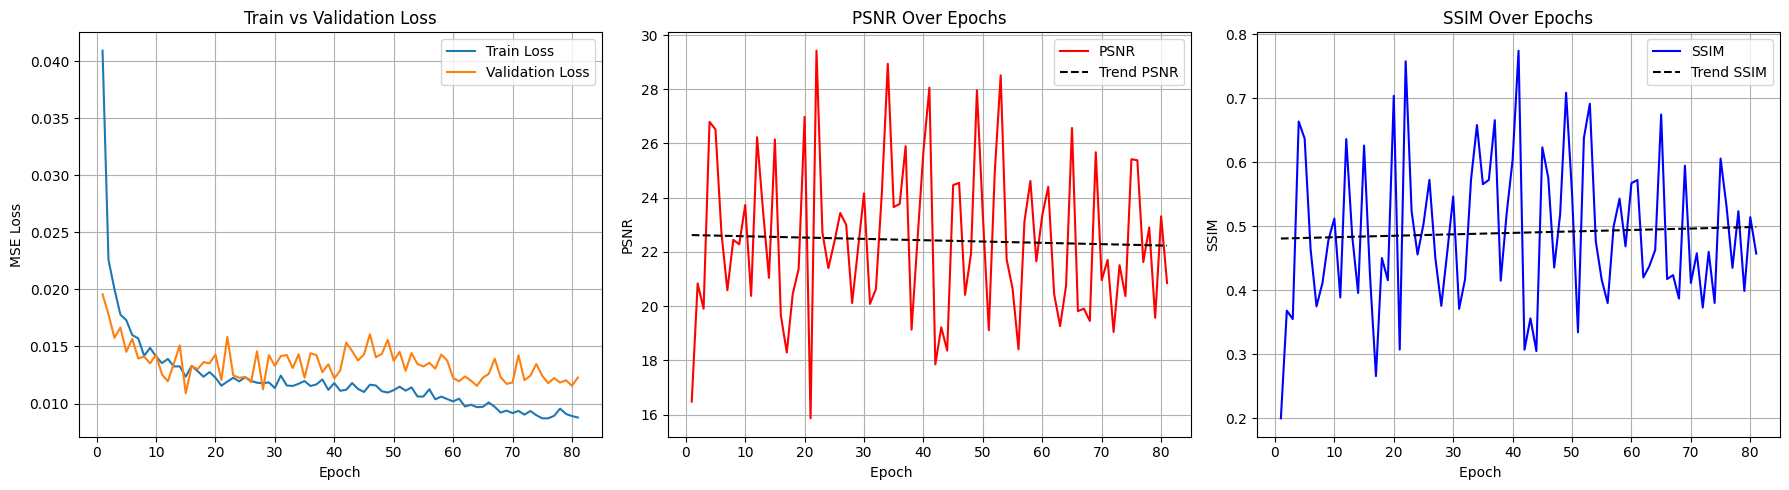
\includegraphics[width=1.0\textwidth]{media/training_results.png}
        \caption{Training Loss, PSNR, and SSIM trends over epochs}
        \label{fig:training_results}
    \end{figure}
\end{frame}

\begin{frame}{Generated Samples from Pure Noise}
    \begin{itemize}
        \item Samples generated from pure noise using the trained model
        \item Visualized to assess the model's generative capabilities
        \item Useful for understanding the model's learned features
        \item Figure \ref{fig:generated_samples_from_pure_noise} shows 10 generated samples to assess the model's performance
    \end{itemize}
\end{frame}

\begin{frame}{Generated Samples Visualization}
    \begin{figure}
        \centering
        % First row
        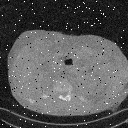
\includegraphics[width=0.15\textwidth]{media/epoch_81_0.png}\hspace{0.5em}
        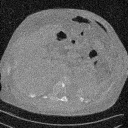
\includegraphics[width=0.15\textwidth]{media/epoch_81_1.png}\hspace{0.5em}
        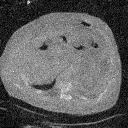
\includegraphics[width=0.15\textwidth]{media/epoch_81_2.png}\hspace{0.5em}
        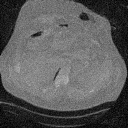
\includegraphics[width=0.15\textwidth]{media/epoch_81_3.png}\hspace{0.5em}
        
\includegraphics[width=0.15\textwidth]{media/epoch_81_4.png}

        \vspace{1em} % Space between rows

        % Second row
        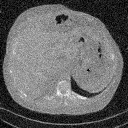
\includegraphics[width=0.15\textwidth]{media/epoch_81_5.png}\hspace{0.5em}
        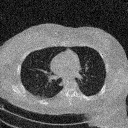
\includegraphics[width=0.15\textwidth]{media/epoch_81_6.png}\hspace{0.5em}
        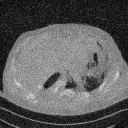
\includegraphics[width=0.15\textwidth]{media/epoch_81_7.png}\hspace{0.5em}
        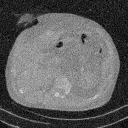
\includegraphics[width=0.15\textwidth]{media/epoch_81_8.png}\hspace{0.5em}
        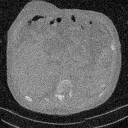
\includegraphics[width=0.15\textwidth]{media/epoch_81_9.png}

        \caption{10 generated samples from pure noise using the trained model at epoch 81.}
        \label{fig:generated_samples_from_pure_noise}
    \end{figure}
\end{frame}
